\documentclass[]{article}
\usepackage{lmodern}
\usepackage{amssymb,amsmath}
\usepackage{ifxetex,ifluatex}
\usepackage{fixltx2e} % provides \textsubscript
\ifnum 0\ifxetex 1\fi\ifluatex 1\fi=0 % if pdftex
  \usepackage[T1]{fontenc}
  \usepackage[utf8]{inputenc}
\else % if luatex or xelatex
  \ifxetex
    \usepackage{mathspec}
  \else
    \usepackage{fontspec}
  \fi
  \defaultfontfeatures{Ligatures=TeX,Scale=MatchLowercase}
\fi
% use upquote if available, for straight quotes in verbatim environments
\IfFileExists{upquote.sty}{\usepackage{upquote}}{}
% use microtype if available
\IfFileExists{microtype.sty}{%
\usepackage{microtype}
\UseMicrotypeSet[protrusion]{basicmath} % disable protrusion for tt fonts
}{}
\usepackage[margin=1in]{geometry}
\usepackage{hyperref}
\hypersetup{unicode=true,
            pdftitle={Road Traffic Accidents Data Analysis using R},
            pdfauthor={Student ID: 201081646},
            pdfborder={0 0 0},
            breaklinks=true}
\urlstyle{same}  % don't use monospace font for urls
\usepackage{color}
\usepackage{fancyvrb}
\newcommand{\VerbBar}{|}
\newcommand{\VERB}{\Verb[commandchars=\\\{\}]}
\DefineVerbatimEnvironment{Highlighting}{Verbatim}{commandchars=\\\{\}}
% Add ',fontsize=\small' for more characters per line
\usepackage{framed}
\definecolor{shadecolor}{RGB}{248,248,248}
\newenvironment{Shaded}{\begin{snugshade}}{\end{snugshade}}
\newcommand{\KeywordTok}[1]{\textcolor[rgb]{0.13,0.29,0.53}{\textbf{{#1}}}}
\newcommand{\DataTypeTok}[1]{\textcolor[rgb]{0.13,0.29,0.53}{{#1}}}
\newcommand{\DecValTok}[1]{\textcolor[rgb]{0.00,0.00,0.81}{{#1}}}
\newcommand{\BaseNTok}[1]{\textcolor[rgb]{0.00,0.00,0.81}{{#1}}}
\newcommand{\FloatTok}[1]{\textcolor[rgb]{0.00,0.00,0.81}{{#1}}}
\newcommand{\ConstantTok}[1]{\textcolor[rgb]{0.00,0.00,0.00}{{#1}}}
\newcommand{\CharTok}[1]{\textcolor[rgb]{0.31,0.60,0.02}{{#1}}}
\newcommand{\SpecialCharTok}[1]{\textcolor[rgb]{0.00,0.00,0.00}{{#1}}}
\newcommand{\StringTok}[1]{\textcolor[rgb]{0.31,0.60,0.02}{{#1}}}
\newcommand{\VerbatimStringTok}[1]{\textcolor[rgb]{0.31,0.60,0.02}{{#1}}}
\newcommand{\SpecialStringTok}[1]{\textcolor[rgb]{0.31,0.60,0.02}{{#1}}}
\newcommand{\ImportTok}[1]{{#1}}
\newcommand{\CommentTok}[1]{\textcolor[rgb]{0.56,0.35,0.01}{\textit{{#1}}}}
\newcommand{\DocumentationTok}[1]{\textcolor[rgb]{0.56,0.35,0.01}{\textbf{\textit{{#1}}}}}
\newcommand{\AnnotationTok}[1]{\textcolor[rgb]{0.56,0.35,0.01}{\textbf{\textit{{#1}}}}}
\newcommand{\CommentVarTok}[1]{\textcolor[rgb]{0.56,0.35,0.01}{\textbf{\textit{{#1}}}}}
\newcommand{\OtherTok}[1]{\textcolor[rgb]{0.56,0.35,0.01}{{#1}}}
\newcommand{\FunctionTok}[1]{\textcolor[rgb]{0.00,0.00,0.00}{{#1}}}
\newcommand{\VariableTok}[1]{\textcolor[rgb]{0.00,0.00,0.00}{{#1}}}
\newcommand{\ControlFlowTok}[1]{\textcolor[rgb]{0.13,0.29,0.53}{\textbf{{#1}}}}
\newcommand{\OperatorTok}[1]{\textcolor[rgb]{0.81,0.36,0.00}{\textbf{{#1}}}}
\newcommand{\BuiltInTok}[1]{{#1}}
\newcommand{\ExtensionTok}[1]{{#1}}
\newcommand{\PreprocessorTok}[1]{\textcolor[rgb]{0.56,0.35,0.01}{\textit{{#1}}}}
\newcommand{\AttributeTok}[1]{\textcolor[rgb]{0.77,0.63,0.00}{{#1}}}
\newcommand{\RegionMarkerTok}[1]{{#1}}
\newcommand{\InformationTok}[1]{\textcolor[rgb]{0.56,0.35,0.01}{\textbf{\textit{{#1}}}}}
\newcommand{\WarningTok}[1]{\textcolor[rgb]{0.56,0.35,0.01}{\textbf{\textit{{#1}}}}}
\newcommand{\AlertTok}[1]{\textcolor[rgb]{0.94,0.16,0.16}{{#1}}}
\newcommand{\ErrorTok}[1]{\textcolor[rgb]{0.64,0.00,0.00}{\textbf{{#1}}}}
\newcommand{\NormalTok}[1]{{#1}}
\usepackage{graphicx,grffile}
\makeatletter
\def\maxwidth{\ifdim\Gin@nat@width>\linewidth\linewidth\else\Gin@nat@width\fi}
\def\maxheight{\ifdim\Gin@nat@height>\textheight\textheight\else\Gin@nat@height\fi}
\makeatother
% Scale images if necessary, so that they will not overflow the page
% margins by default, and it is still possible to overwrite the defaults
% using explicit options in \includegraphics[width, height, ...]{}
\setkeys{Gin}{width=\maxwidth,height=\maxheight,keepaspectratio}
\IfFileExists{parskip.sty}{%
\usepackage{parskip}
}{% else
\setlength{\parindent}{0pt}
\setlength{\parskip}{6pt plus 2pt minus 1pt}
}
\setlength{\emergencystretch}{3em}  % prevent overfull lines
\providecommand{\tightlist}{%
  \setlength{\itemsep}{0pt}\setlength{\parskip}{0pt}}
\setcounter{secnumdepth}{5}
% Redefines (sub)paragraphs to behave more like sections
\ifx\paragraph\undefined\else
\let\oldparagraph\paragraph
\renewcommand{\paragraph}[1]{\oldparagraph{#1}\mbox{}}
\fi
\ifx\subparagraph\undefined\else
\let\oldsubparagraph\subparagraph
\renewcommand{\subparagraph}[1]{\oldsubparagraph{#1}\mbox{}}
\fi

%%% Use protect on footnotes to avoid problems with footnotes in titles
\let\rmarkdownfootnote\footnote%
\def\footnote{\protect\rmarkdownfootnote}

%%% Change title format to be more compact
\usepackage{titling}

% Create subtitle command for use in maketitle
\newcommand{\subtitle}[1]{
  \posttitle{
    \begin{center}\large#1\end{center}
    }
}

\setlength{\droptitle}{-2em}

  \title{Road Traffic Accidents Data Analysis using R}
    \pretitle{\vspace{\droptitle}\centering\huge}
  \posttitle{\par}
    \author{Student ID: 201081646}
    \preauthor{\centering\large\emph}
  \postauthor{\par}
    \date{}
    \predate{}\postdate{}
  
\usepackage{float} \floatplacement{figure}{H}

\begin{document}
\maketitle

\section{Introduction}\label{introduction}

This report is the second assessment of the \textbf{MATH5741M
Statistical Theory and Methods} module. Its aim is to answer three
questions through inferential statistical analysis regarding a road
traffic accidents dataset from the UK Department for Transport.

All the analysis has been done using \textbf{R} (programming language)
and is code reproducible. To see the complete \textbf{R} coding process
and outputs visit
\url{https://github.com/eugenividal/Road-Traffic-Accidents-Data-Analysis}

\section{Results}\label{results}

\subsection{Question 1}\label{question-1}

In this question, first, we are asked to draw a boxplot to compare the
number of vehicles involved in urban areas with the number invlolved in
rural areas.

\url{http://www.jbstatistics.com/pooled-variance-t-tests-and-confidence-intervals-an-example/}

To plot the boxplot, we first remove the unallocated values. Next, we
visualise the data to analyse if it is normal (histogram 1). Because it
is very skewed to the right, we take the log10 and see that it
substantially improves (histogram 2).

\begin{Shaded}
\begin{Highlighting}[]
\CommentTok{# show table of values}
\KeywordTok{table}\NormalTok{(xx_area$Number_of_Vehicles)}
\end{Highlighting}
\end{Shaded}

\begin{verbatim}
## 
##      1      2      3      4      5      6      7      8      9     10 
##  59770 117114  17002   3516    819    262     83     40     18      8 
##     11     12     13     15     17     18     20 
##      4      2      1      1      1      2      2
\end{verbatim}

\begin{figure}[H]

{\centering 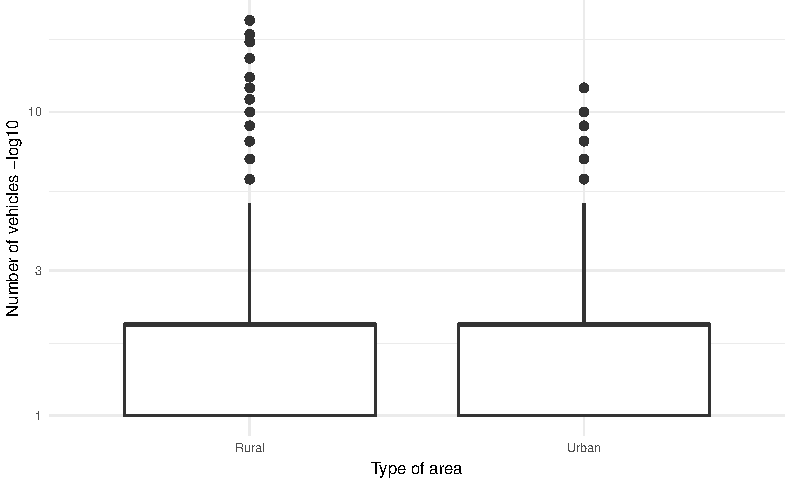
\includegraphics{READMEv2_files/figure-latex/fig-1} 

}

\caption{Histograms}\label{fig:fig}
\end{figure}

\begin{figure}[H]

{\centering 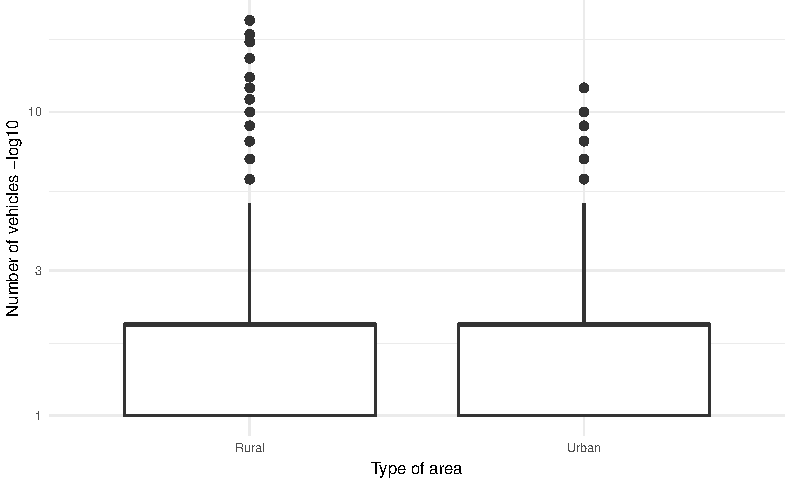
\includegraphics{READMEv2_files/figure-latex/fig2-1} 

}

\caption{Number of vehicles involved grouped by type of area}\label{fig:fig2}
\end{figure}

Secondly, we have to carry out a test to investigate wheter the average
number of vehicles in an accident differs per type of area.

For this, using the transformation we perform a \textbf{pooled variance
test}. We assume that \(\sigma_{1}^{2}\) = \(\sigma_{2}^{2}\) =
\(\sigma^{2}\)

\url{http://www.jbstatistics.com/inference-for-two-means-introduction/}

\[H_{0}: \mu_{urban} = \mu_{rural}\;\;\;vs.\;\;\;H_{1}: \mu_{urban} \neq \mu_{rural}\]

They are not about the same, should we continue with a two sample test
which assumes equal variance? The independent t-test assumes the
variances of the two groups you are measuring are equal in the
population. If your variances are unequal, this can affect the Type I
error rate. The assumption of homogeneity of variance can be tested
using Levene's Test of Equality of Variances.

\begin{Shaded}
\begin{Highlighting}[]
\CommentTok{# pooled variance test}
\CommentTok{#t.test(xx[])}
\end{Highlighting}
\end{Shaded}

In conclusion, we can say that

\subsection{Question 2}\label{question-2}

In this question, first, we have to investigate whether the frequency of
accidents varies by day of the week using the suitable statistical
hypothesis test.

For this, we apply a \textbf{chi-squared test}.

\url{http://www.jbstatistics.com/chi-square-tests-for-one-way-tables/}

\begin{Shaded}
\begin{Highlighting}[]
\CommentTok{# hypothesis per each day}
\KeywordTok{ggplot}\NormalTok{(xx, }\KeywordTok{aes}\NormalTok{(}\DataTypeTok{x=}\NormalTok{Day_of_Week))+}\KeywordTok{geom_bar}\NormalTok{() +}
\StringTok{  }\KeywordTok{theme}\NormalTok{(}\DataTypeTok{axis.text.x =} \KeywordTok{element_text}\NormalTok{(}\DataTypeTok{angle =} \DecValTok{45}\NormalTok{, }\DataTypeTok{hjust=}\DecValTok{1}\NormalTok{))}
\end{Highlighting}
\end{Shaded}

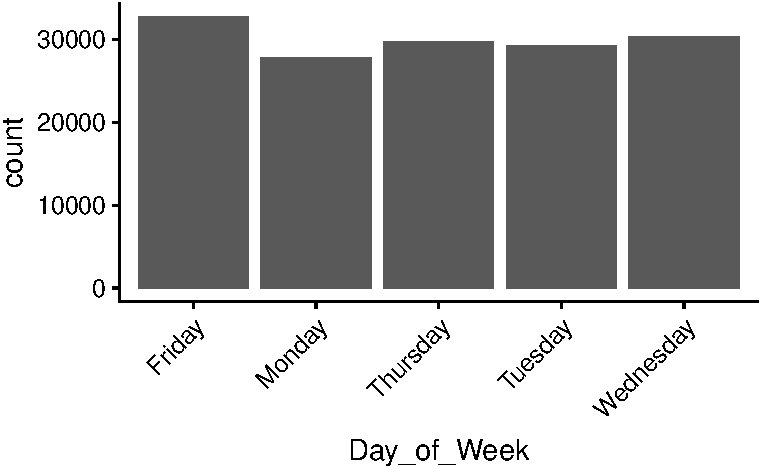
\includegraphics{READMEv2_files/figure-latex/unnamed-chunk-13-1.pdf}

Next, we are required to do the same test using only week-days
(excluding Saturday and Sunday).

\begin{Shaded}
\begin{Highlighting}[]
\CommentTok{# Select data using only week-days}
\NormalTok{week_days <-}\StringTok{ }\NormalTok{xx%>%}
\StringTok{  }\KeywordTok{select}\NormalTok{(Day_of_Week)%>%}
\StringTok{  }\KeywordTok{filter}\NormalTok{(!Day_of_Week %in%}\StringTok{ }\KeywordTok{c}\NormalTok{(}\StringTok{"Saturday"}\NormalTok{, }\StringTok{"Sunday"}\NormalTok{))}
\end{Highlighting}
\end{Shaded}

\begin{verbatim}
## Warning: package 'bindrcpp' was built under R version 3.4.4
\end{verbatim}

\begin{Shaded}
\begin{Highlighting}[]
\KeywordTok{table}\NormalTok{(week_days)}
\end{Highlighting}
\end{Shaded}

\begin{verbatim}
## week_days
##    Friday    Monday  Thursday   Tuesday Wednesday 
##     32738     27812     29738     29219     30373
\end{verbatim}

\begin{Shaded}
\begin{Highlighting}[]
\KeywordTok{ggplot}\NormalTok{(week_days, }\KeywordTok{aes}\NormalTok{(}\DataTypeTok{x=}\NormalTok{Day_of_Week))+}\KeywordTok{geom_bar}\NormalTok{() +}
\StringTok{  }\KeywordTok{theme}\NormalTok{(}\DataTypeTok{axis.text.x =} \KeywordTok{element_text}\NormalTok{(}\DataTypeTok{angle =} \DecValTok{45}\NormalTok{, }\DataTypeTok{hjust=}\DecValTok{1}\NormalTok{)) }
\end{Highlighting}
\end{Shaded}

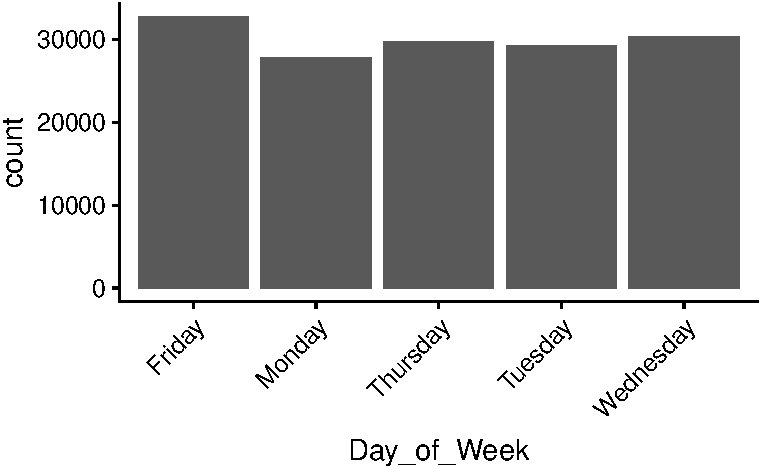
\includegraphics{READMEv2_files/figure-latex/unnamed-chunk-14-1.pdf}

\begin{Shaded}
\begin{Highlighting}[]
\CommentTok{# hypothesis per each day using only week-days}
\end{Highlighting}
\end{Shaded}

\subsection{Question 3}\label{question-3}

Finally, in question 3, we are asked to compute a 95\% confidence
interval for the expected (mean) number of accidents which occur on a
Monday.

Look at example in p.62 to answer this:

\begin{itemize}
\item
  The data is clearly not normal. The distribution is discrete and very
  skewed to the right. The table of values is:
\item
  The sample is huge (\emph{n}= 198,735) so the central limit theorem
  stats that the sample mean in normallly distributed (even when the
  data are not).
\item
  However, we need to think - for which population are we estimating a
  mean for?.
\end{itemize}

Is this a simple t-distribution confidence interval? WE could say that
because the sample is that bing could be just a normal confidence
interval?

I need to create calculate the mean of accidents on Mondays, so per each
Monday which is the number of accidents expected. How to do that?

\begin{Shaded}
\begin{Highlighting}[]
\CommentTok{# Select data using only week-days}
\NormalTok{Mondays<-}\StringTok{ }\NormalTok{xx%>%}
\StringTok{  }\KeywordTok{select}\NormalTok{(count, Day_of_Week)%>%}
\StringTok{  }\KeywordTok{group_by}\NormalTok{(Day_of_Week)%>%}\StringTok{ }
\StringTok{  }\KeywordTok{summarise}\NormalTok{(}\DataTypeTok{sum =} \KeywordTok{sum}\NormalTok{(count))}
\end{Highlighting}
\end{Shaded}

\begin{Shaded}
\begin{Highlighting}[]
\CommentTok{#t.test(Mondays, conf.level = 0.95)$conf.int}
\end{Highlighting}
\end{Shaded}

\section{Bibliography}\label{bibliography}

The resources used to carry out this project were:

\begin{itemize}
\tightlist
\item
  Balka, J. 2013. JBStatistics: Making Statistics Make Sense. Available
  from: \url{http://www.jbstatistics.com}.
\item
  Lane, D.M. 2018. Online Statistics Education: An Interactive
  Multimedia Course of Study. Available from:
  \url{http://onlinestatbook.com/}.
\item
  Taylor, C. 2017. MATH5741M: Statistical Theory and Methods. Outline
  Lecture Notes.
\item
  Yau, C. 2018. R tutorial: an R introduction to statistics. Available
  from: \url{http://www.r-tutor.com}
\end{itemize}


\end{document}
